%%%%%%%%%%%%%%%%%%%%%%%%%%%%%%%%%%%%%%%%%%%%%%%%%%%%%%%%%%%%%%%%%%%%%%%%%%%%%%%

\section*{\large Exercício 2}
\addcontentsline{toc}{chapter}{\protect\numberline{}\large Exercício 2}%

Mostrarei que

\begin{equation*}
\text{FT}[\alpha f + g](t) = \alpha \text{FT}[f(t)] + \text{FT}[g(t)].
\end{equation*}

\textbf{Resolução:}

Da Eq. 1:

\begin{align*}
\text{FT}[\alpha f + g](t) &= \frac{1}{2 \pi} \int_{-\infty}^{+\infty} (\alpha \hat{f}(\xi) + \hat{g}(\xi)) e^{\imath \xi t} d\xi \\[10pt]
&= \alpha \frac{1}{2 \pi} \int_{-\infty}^{+\infty} \hat{f}(\xi)e^{\imath \xi t} d\xi + \frac{1}{2 \pi} \int_{-\infty}^{+\infty} \hat{g}(\xi) e^{\imath \xi t} d \xi \\[10pt]
 &= \alpha \text{FT}[f(t)] + \text{FT}[g(t)]. \tag*{(Q.E.D.)}
\end{align*}

A Figura 2.1 abaixo ilustra a linearidade da FT, que é o significado da resolução acima. Duas funções cosseno, uma de período igual a dez ($f_{1}$) e outra de período igual a vinte ($f_{2}$) são somadas para gerar uma terceira função ($f_{3}$). A parte real de suas Transformadas de Fourier ($\hat{f}_{1}, \hat{f}_{2}$ e $\hat{f}_{3}$) estão à direita, e o último plot (canto direito inferior) atesta que $\hat{f}_{3} = \hat{f}_{1} + \hat{f}_{2}$.

% EXEMPLO PARA ADICIONAR FIGURA
\begin{figure}[ht!]
	%\caption{Exemplo da linearidade da FT.}
	\legenda{Figura 2.1: Exemplo da linearidade da FT.}
	\vspace{0mm}	% acrescentar o espaçamento vertical apropriado entre o título e a borda superior da figura
	\begin{center}
		\resizebox{\textwidth}{!}{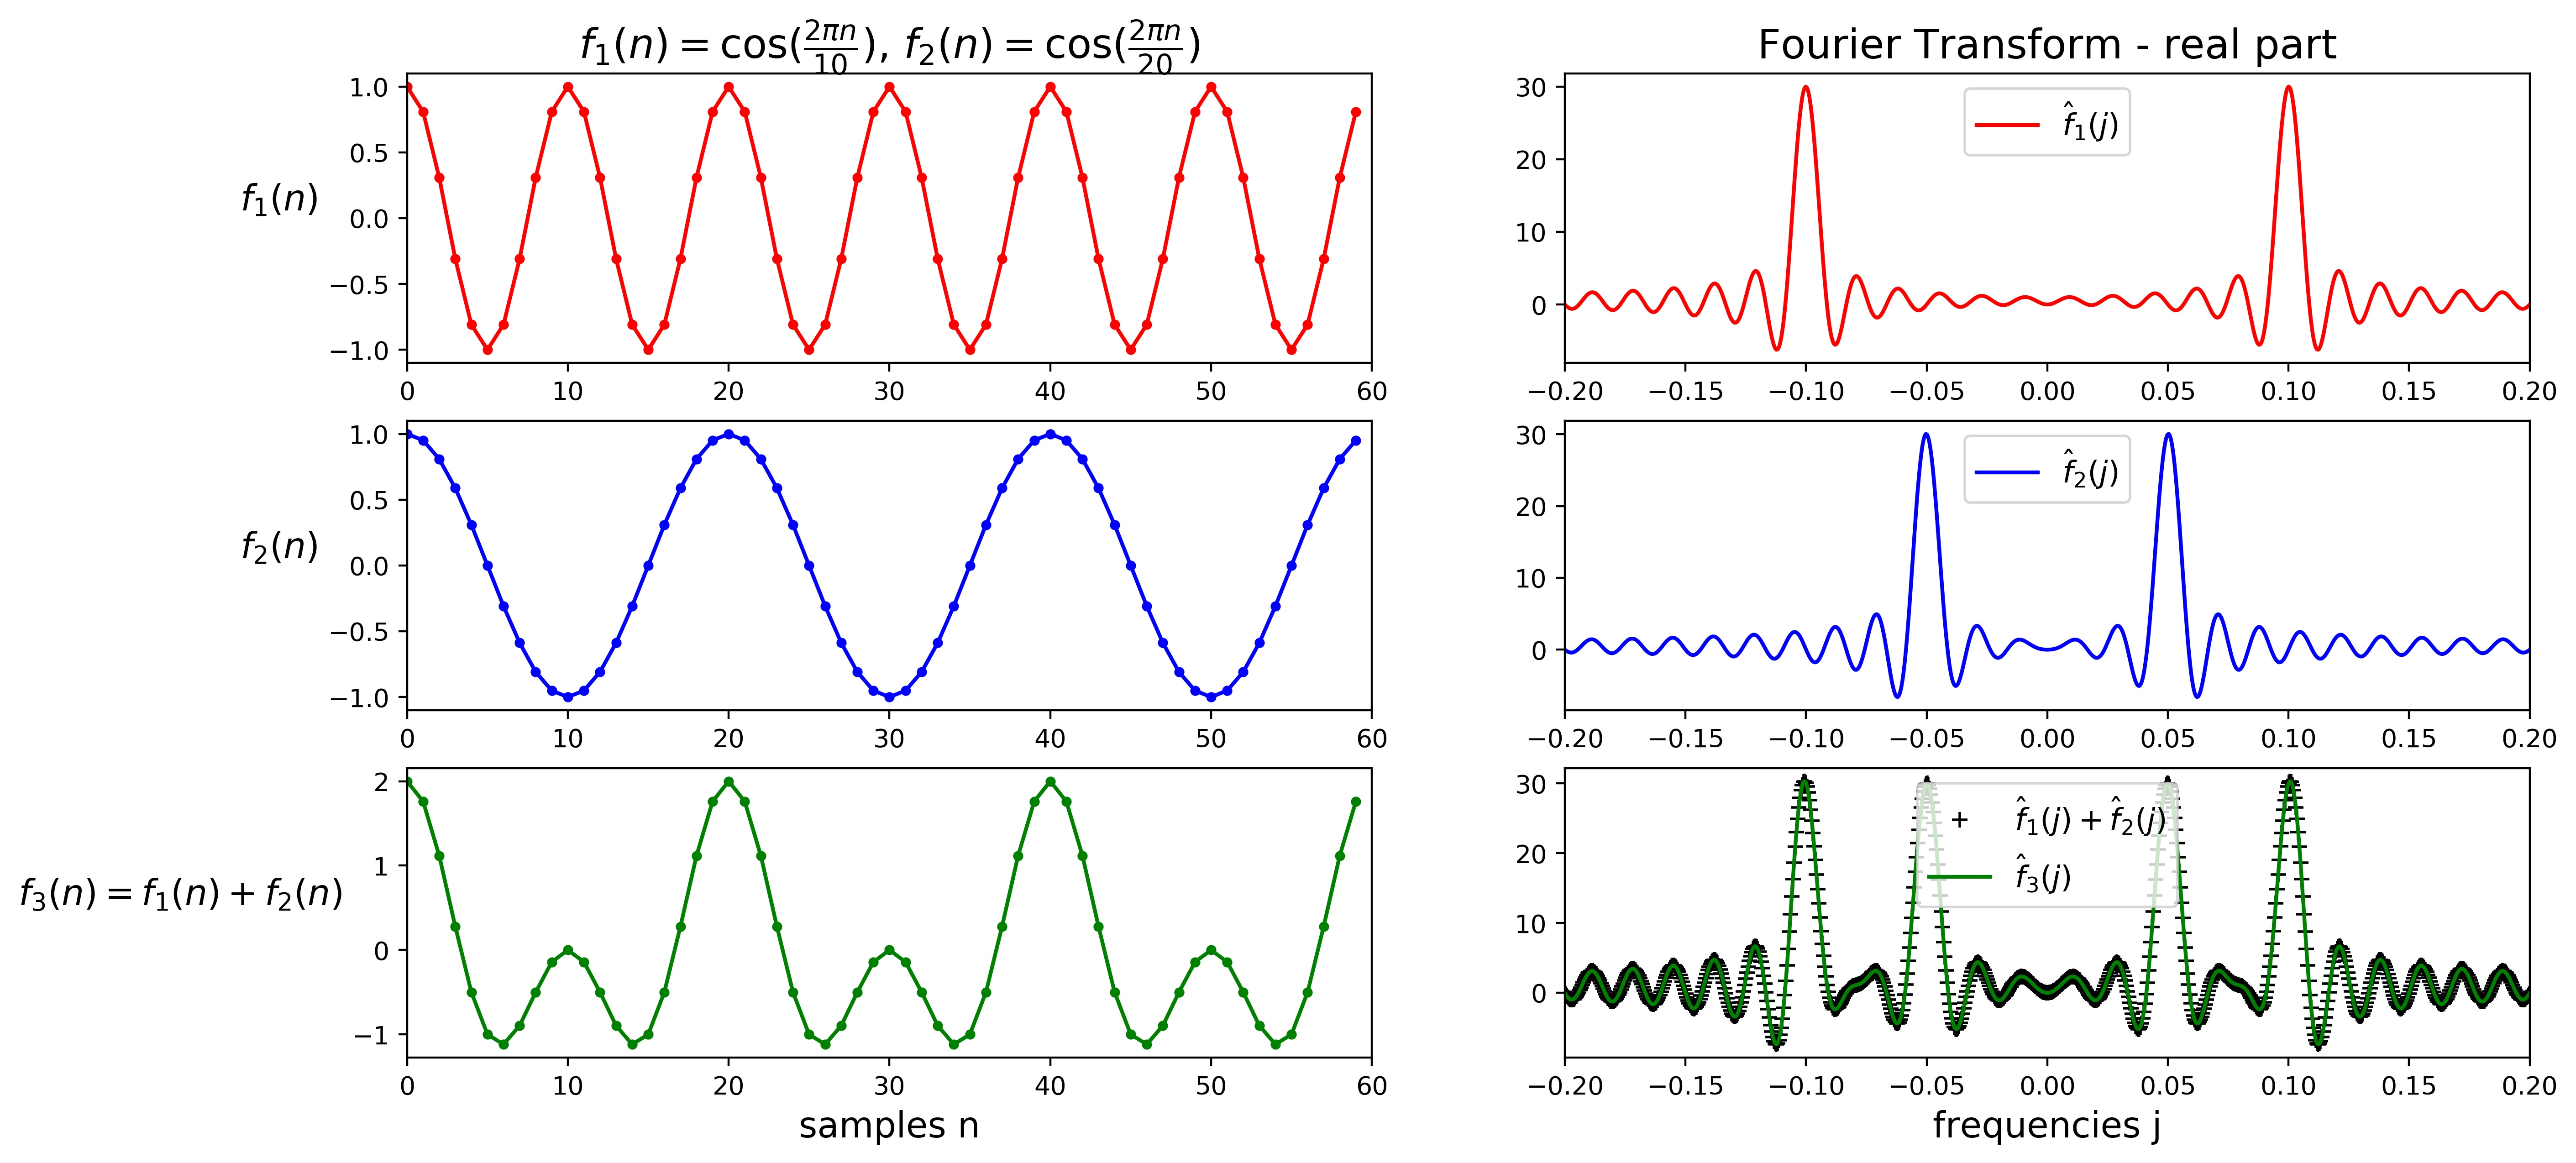
\includegraphics{../scripts/exercicio2/exemplo_FT_linear.jpg}}		
	\end{center}
	\vspace{-2mm}	% acrescentar o espaçamento vertical apropriado entre a borda inferior da figura e a legenda ou a fonte quando não há legenda (o valor pode ser negativo para subir)
	%\legenda{Figura 2.1: Exemplo da linearidade da FT.}	% legenda - para deixar sem legenda usar comando \legenda{} (nunca deve-se comentar o comando \legenda)
	%\label{ex1_fig1}
	%\FONTE{}	% fonte consultada (elemento obrigatório, mesmo que seja produção do próprio autor)
\end{figure}
